%!TEX root = ../Thesis.tex
\chapter{Preface}
This bachelor thesis was written at the department of Automation and Control at the Technical University of Denmark in fulfilment of the requirements for acquiring a bachelor degree in Electrical Engineering.\\
\\
\noindent
This project is an innovation project, which pushes the boundaries of relative low cost technology. There is an old Danish saying that "The higher you fly, the further you fall". Innovation project are about being willing to take a high risk, of falling deep, to achieve results no one thought was possible. If every innovation project succeeded, it is not innovation -- but only a further development of existing technology. To achieve an innovative goal, you have to set a goal 110 per cent higher of what you expect to achieve and afterwards be fair in sentencing if missing the target.\\
Innovation is an iterative process where learning comes from both successes and failures. 
\\
\noindent
The target audience for this thesis is students/staff with an electrical engineering background who are interested in this project and the focus is on how they can benefit from this work using the method and results.    

\vfill

{
\centering
    \thesislocation{}, \today\\[1cm]
    \hspace{3cm}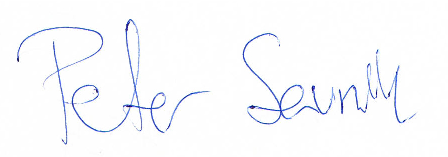
\includegraphics[scale=1]{Signature}\\[1cm]
\begin{flushright}
    \thesisauthor{}
\end{flushright}
}